\section{Diffraction des ondes}

Tant qu'une onde ne change pas de milieu ou ne rencontre pas
d'obstacles, elle se propage en ligne droite. Que se passe-t-il
lorsqu'elle passe près d'obstacles ?

Nous entendons facilement au milieu de la classe, des bruits venant du
couloir lorsque la porte est ouverte. De même, nous percevons très bien
des bruits provenant de l'extérieur et ce par une fenêtre ouverte.

Une onde ne devrait-elle pas être arrêtée par un obstacle~?

\subsection{Observations avec la cuve à onde. }

\subsubsection{Passage à travers une fente}

Considérons des ondes planes, produites dans une cuve à onde, come nous
l'avons vu au cours.

Les images ci-dessous sont vues de haut, les ondes se propagent du bas
vers le haut.

Nous les voyons passer à travers une fente \emph{de largeur que
nous noterons $x$}.

\paragraph{Observation avec la cuve à ondes}

\subparagraph{Schémas}

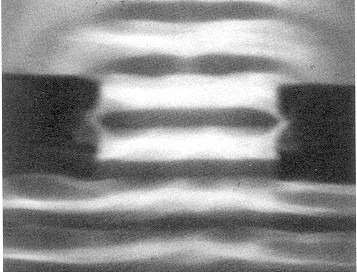
\includegraphics[width=4.546cm,height=3.468cm]{Pictures/1000000100000165000001102080785BE3C607F4.png}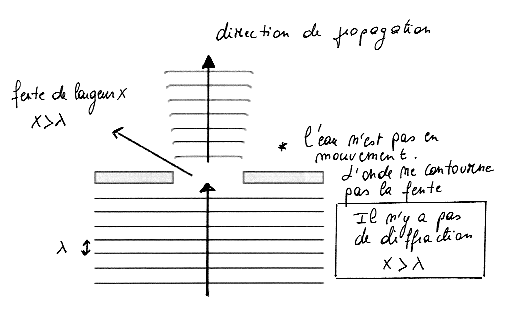
\includegraphics[width=7.895cm,height=6.091cm]{Pictures/10000001000002060000013F9C2B947BF01F091E.png}

\begin{figure}
\centering
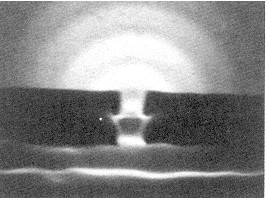
\includegraphics[width=5.166cm,height=3.817cm]{Pictures/100000010000010C000000C6588B9A00B1CFD310.png}
\caption{}
\end{figure}

\begin{figure}
\centering
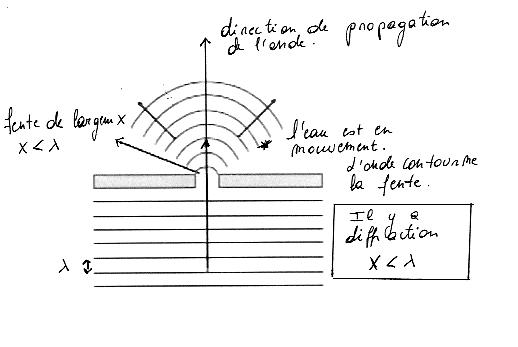
\includegraphics[width=8.348cm,height=5.408cm]{Pictures/10000001000002060000015BBB1606831ABACDE3.png}
\caption{}
\end{figure}

Comment expliquer que nous entendions facilement au milieu
de la classe, des bruits venant du couloir lorsque la porte est
ouverte~alors que nous savons que la propagation des ondes est
rectiligne~?

\subsection{Principe de Huygens.}

Pour expliquer ces observations, Huygens a élaboré une théorie
ondulatoire (1818) qui permet d'expliquer ce phénomène de diffraction.

TODO ajouter biographie de Huygens

Le principe de Huygens peut être énoncé comme~: « tout point atteint par une onde se
comporte comme une nouvelle source d'ondes circulaires de même
fréquence, c'est-à-dire que ce point génère des ondes circulaires de
même fréquence. »

\subsubsection{Une onde circulaire se propage de façon circulaire }

\begin{figure}
\centering
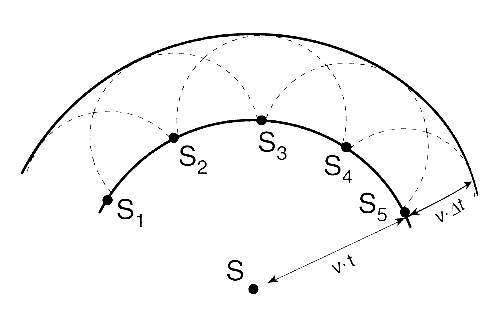
\includegraphics[width=5.369cm,height=3.551cm]{Pictures/10000001000001E8000001439B3D312A195F0A9A.png}
\caption{}
\end{figure}

Imaginons une goutte d'eau qui tombe à la surface de l'eau en un point
S. Une onde circulaire va se propager et atteindre les points S1, S2,
S3, S4, \ldots. Chacun de ces points atteints par l'onde va générer des
ondes circulaires de même fréquence (et donc de même longueur d'onde si
le milieu est inchangé).

C'est ainsi qu'une onde circulaire continue à se propager de façon
circulaire.

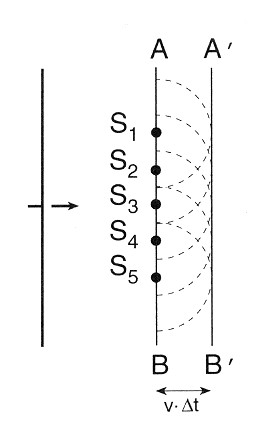
\includegraphics[width=3.461cm,height=5.323cm]{Pictures/1000000100000118000001AF621E98E90630327B.png}\emph{b)
Pourquoi une onde plane continue-t-elle à se propager de façon plane~? }

Soit une tige plane produisant des ondes planes. Le front d'ondes arrive
sur la ligne AB. En vertu du principe de Huygens, chaque point du
segment AB (S1, S2, S3, S4, S5) produit des ondes circulaires et nous
voyons que toutes ces ondes vont former finalement sur le segment A'B'
une onde plane.

Une onde plane se propage donc en restant une onde plane.
\subsubsection{Passage (ou non) derrière un obstacle. }

Au lieu de faire passer une onde à travers une fente, nous pouvons aussi
lui faire rencontrer un obstacle.

Nous l'avons observé avec la cuve à onde et vu que~:

\begin{itemize}
\item  Si les dimensions de l'obstacle sont grandes devant la longueur
  d'onde, l'onde ne contourne pas l'obstacle.
\item  Si les dimensions de l'obstacle sont petites devant la longueur
  d'onde, l'onde contourne l'obstacle.
\end{itemize}

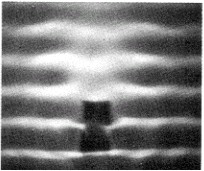
\includegraphics[width=4.731cm,height=3.974cm]{Pictures/10000001000000CC000000ABB81AAF52FD11C7D3.png}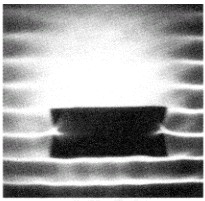
\includegraphics[width=4.128cm,height=4.046cm]{Pictures/10000001000000CD000000C9CF0691AC9C53D126.png}

\subsubsection{Conclusions}

\textbf{La diffraction est le comportement des
}\href{https://fr.wikipedia.org/wiki/Onde}{\emph{\emph{\textbf{ondes}}}}\textbf{
lorsqu'elles rencontrent un obstacle ou une ouverture. }

\textbf{Plus la longueur d'une onde est grande par rapport aux
dimensions de l'obstacle (ou la largeur de l'ouverture), plus cette onde
aura de facilité à contourner (à envelopper) l'obstacle.}
\subsection{3.3. Applications }

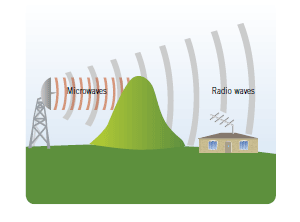
\includegraphics[width=7.108cm,height=5.267cm]{Pictures/100000010000012C000000DEA5F8143A7ED3E9C1.png}\emph{\textbf{a)
Réception des ondes radio en fonction de la longueur d'onde}

Ainsi les grandes ondes radio (longueurs d'onde hectométriques et
kilométriques) peuvent pénétrer dans le moindre recoin de la surface
terrestre tandis que les retransmissions de télévision par satellite
(courtes longueurs d `ondes) ne sont possibles que si l'antenne de
réception «~voit~» le satellite.

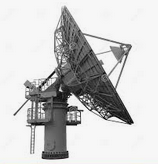
\includegraphics[width=5.586cm,height=5.808cm]{Pictures/100000010000009E000000A4B38E4E23C937303B.png}\emph{\textbf{b)
Les antennes paraboliques}

Pourquoi les réflecteurs des antennes paraboliques sont-ils de si
grandes dimensions~?

\begin{figure}
\centering
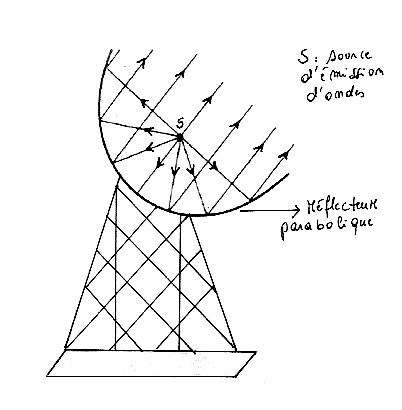
\includegraphics[width=5.166cm,height=5.269cm]{Pictures/10000001000001920000019ACA6FE085C34366DF.png}
\caption{}
\end{figure}

En plaçant la source S au foyer du réflecteur parabolique, on produit,
par réflexion, un faisceau parallèle de telle sorte que presque toute
l'énergie partira dans une seule direction (vers un satellite, vers un
relais, \ldots).

Il faut cependant que la longeur d'onde de l'onde émise soit plus petite
que le diamètre du réflecteur pour \emph{\textbf{éviter la diffraction}
(et donc que l'onde ne contourne pas le réflecteur)\subsection{(x}\textbf{}\textbf{).}

Le remarque est identique pour des antennes paraboliques réceptrices
d'ondes.
\subsection{c) Echolocation}

Certains animaux, dauphins, chauve-souris) émettent des ondes
acoustiques et ensuite captent les ondes réfléchies par les objets
environnants, détectant ainsi les obstacles et proies éventuelles. Il
faut pour cela que la longueur d'onde soit inférieure aux dimensions de
l'obstacle à détecter. (Il faut donc ici peu de diffraction et le
maximum de réflexion).

En effet, si la longueur d'onde était plus grande que les objets, il y
aurait trop de diffraction derrière celui-ci et il y aurait peu d'onde
réfléchie.

C'est pour cela que les dauphins et chauve-souris émettent des ondes
acoustiques de fréquence élevée et donc de longueur d'onde très faible
pour \emph{\textbf{éviter la diffraction (x}\textbf{}\textbf{).}}. Ces
ondes seront donc des ultrasons.

C'est aussi le principe du sonar et du radar.

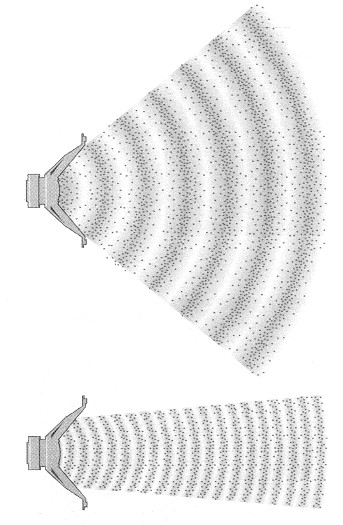
\includegraphics[width=5.36cm,height=7.996cm]{Pictures/10000001000001570000020D95DCA793B8E9458C.png}\emph{\textbf{d)
Les dimensions d'un haut-parleur}

Un haut-parleur se comporte comme une fente traversée par une onde.

Un haut-parleur doit envoyer une onde de grande longueur d'onde devant
le diamètre du haut-parleur \emph{\textbf{(x}\textbf{}\textbf{) pour
favoriser la diffraction}} de façon à diffuser les sons dans un cône
assez ouvert.
\subsection{EXERCICES SUR LE PHENOMENE DE DIFFRACTION}

\hypertarget{exercice-1}{%
\section{\texorpdfstring{\emph{EXERCICE
1}}{EXERCICE 1}}\label{exercice-1}

\hypertarget{peut-on-recevoir-derriuxe8re-une-colline-de-100-muxe8tres-de-largeur-des-ondes-radio-de-30-000-hz-si-luxe9metteur-se-trouve-au-bas-de-la-colline}{%
\section{\texorpdfstring{Peut-on recevoir derrière une colline de 100
mètres de largeur des ondes radio de 30 000 Hz si l'émetteur se trouve
au bas de la colline~?
}{Peut-on recevoir derrière une colline de 100 mètres de largeur des ondes radio de 30 000 Hz si l'émetteur se trouve au bas de la colline~? }}\label{peut-on-recevoir-derriuxe8re-une-colline-de-100-muxe8tres-de-largeur-des-ondes-radio-de-30-000-hz-si-luxe9metteur-se-trouve-au-bas-de-la-colline}

\begin{quote}\subsection{EXERCICE 2}
\end{quote}

\begin{quote}
Les chauves-souris émettent des sons de haute fréquence pour situer les
objets qui les entourent. La fréquence la plus élevée émise par une
espèce de chauve-souris est égale à 50 kHz. Quelles sont les dimensions
minimales des insectes qu'elle pourra détecter fiablement~?
\end{quote}

\begin{figure}
\centering
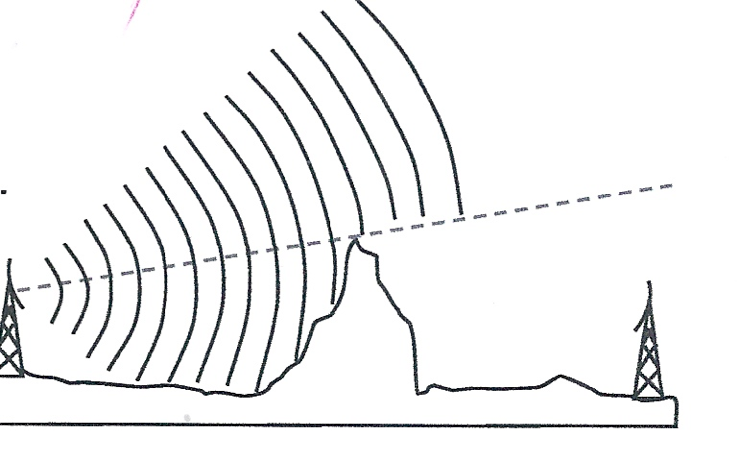
\includegraphics[width=4.445cm,height=2.787cm]{Pictures/10000001000002E4000001CE9CDB74834F100431.png}
\caption{}
\end{figure}
\subsection{EXERCICE 3}

\begin{quote}
Une station radio émet sur une fréquence de 101 MHz.
\end{quote}

\begin{quote}
Les habitants d'un village situé au fond d'une vallée, dont les
dimensions sont de l'ordre du kilomètre vont-il bien capter cette
station ?
\end{quote}

\begin{quote}\subsection{EXERCICE 4}
\end{quote}

\begin{quote}
Pour se situer par rapport à d'éventuels obstacles, un dauphin produit
des ultrasons de fréquence f=40 kHz.
\end{quote}

\begin{quote}
Quelle est la dimension de la plus petite proie que le dauphin peut
attraper, les yeux fermés ?
\end{quote}

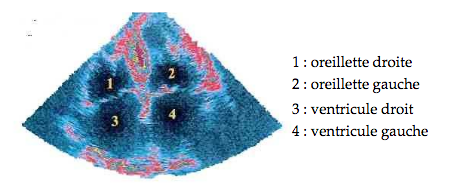
\includegraphics[width=10.084cm,height=4.142cm]{Pictures/10000001000001D1000000BF0020819CCFE94127.png}\emph{\textbf{EXERCICE
5 }

Des ondes ultrasonores de fréquence 2,00 MHz sont utilisées pour
réaliser l'échographie du cœur. Dans les tissus cardiaques, leur vitesse
de propagation est de l'ordre de 1,5 km/s.

Ces ondes peuvent-elle être diffractées par le cœur ?

\begin{figure}
\centering
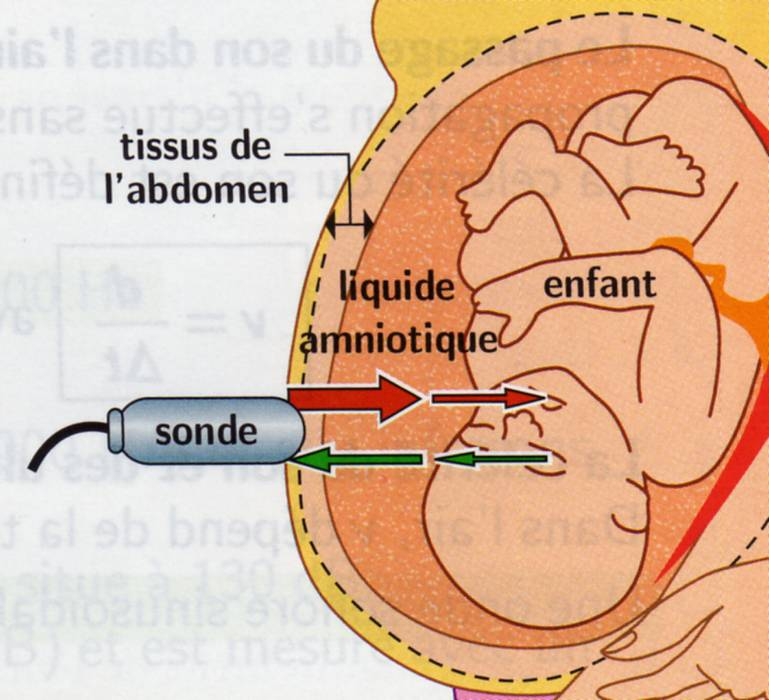
\includegraphics[width=5.009cm,height=4.621cm]{Pictures/1000000000000301000002BCCF7FB7734DEACB0A.jpg}
\caption{}
\end{figure}
\subsection{EXERCICE 6}

L'échographie est une technique d'imagerie médicale fréquemment utilisée
notamment pour suivre le développement des fœtus et la détection
d~`anomalies éventuelles.

Un examen échographique est réalisé avec une sonde qui émet des
impulsions ultrasonores de fréquence 4 MHz. La vitesse des ondes dans le
milieu concerné est de 1540 m/s.

Cet examen fonctionne comme un sonar en numérisant à la fin le signal
réfléchi en image.

\begin{enumerate}
\def\labelenumi{\alph{enumi})}
\tightlist
\item
  Explique pourquoi on utilise des ultrasons plutôt que des ondes de
  plus petite fréquence
\end{enumerate}

\begin{enumerate}
\def\labelenumi{\alph{enumi})}
\tightlist
\item
  L'appareil décrit permet-il de détecter un embryon qui ne mesure que
  5mm~? Justifie ta réponse
\end{enumerate}
\subsection{EXERCICES SUR LE PHENOMENE DE DIFFRACTION}

\hypertarget{exercice-1-1}{%
\section{\texorpdfstring{\emph{EXERCICE
1}}{EXERCICE 1}}\label{exercice-1-1}

\hypertarget{section}{%
\section{}\label{section}

\hypertarget{peut-on-recevoir-derriuxe8re-une-colline-de-100-muxe8tres-de-largeur-des-ondes-radio-de-30-000-hz-si-luxe9metteur-se-trouve-au-bas-de-la-colline-1}{%
\section{\texorpdfstring{Peut-on recevoir derrière une colline de 100
mètres de largeur des ondes radio de 30 000 Hz si l'émetteur se trouve
au bas de la colline~?
}{Peut-on recevoir derrière une colline de 100 mètres de largeur des ondes radio de 30 000 Hz si l'émetteur se trouve au bas de la colline~? }}\label{peut-on-recevoir-derriuxe8re-une-colline-de-100-muxe8tres-de-largeur-des-ondes-radio-de-30-000-hz-si-luxe9metteur-se-trouve-au-bas-de-la-colline-1}

\begin{quote}\subsection{EXERCICE 2}
\end{quote}

Les chauves-souris émettent des sons de haute fréquence pour situer les
objets qui les entourent. La fréquence la plus élevée émise par une
espèce de chauve-souris est égale à 50 kHz. Quelles sont les dimensions
minimales des insectes qu'elle pourra détecter fiablement~?
\subsection{EXERCICE 3}

\begin{quote}
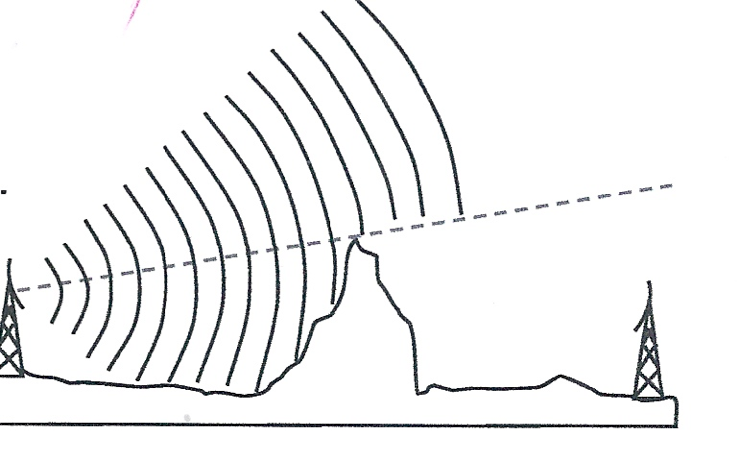
\includegraphics[width=4.445cm,height=2.787cm]{Pictures/10000001000002E4000001CE9CDB74834F100431.png}Une
station radio émet sur une fréquence de 101 MHz.
\end{quote}

\begin{quote}
Les habitants d'un village situé au fond d'une vallée, dont les
dimensions sont de l'ordre du kilomètre vont-il bien capter cette
station ?
\end{quote}
\subsection{EXERCICE 4}

Pour se situer par rapport à d'éventuels obstacles, un dauphin produit
des ultrasons de fréquence f=40 kHz.

Quelle est la dimension de la plus petite proie que le dauphin peut
attraper, les yeux fermés ?
\subsection{EXERCICE 5 }

\begin{figure}
\centering
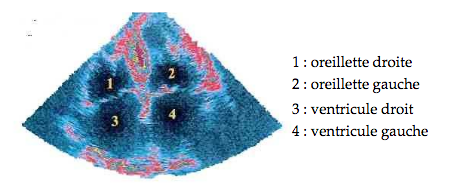
\includegraphics[width=10.084cm,height=4.142cm]{Pictures/10000001000001D1000000BF0020819CCFE94127.png}
\caption{}
\end{figure}

Des ondes ultrasonores de fréquence 2,00 MHz sont utilisées pour
réaliser l'échographie du cœur. Dans les tissus cardiaques, leur vitesse
de propagation est de l'ordre de 1,5 km/s.

Ces ondes peuvent-elle être diffractées par le cœur ?
\subsection{EXERCICE 6}

L'échographie est une technique d'imagerie médicale fréquemment utilisée
notamment pour suivre le développement des fœtus et la détection
d~`anomalies éventuelles.

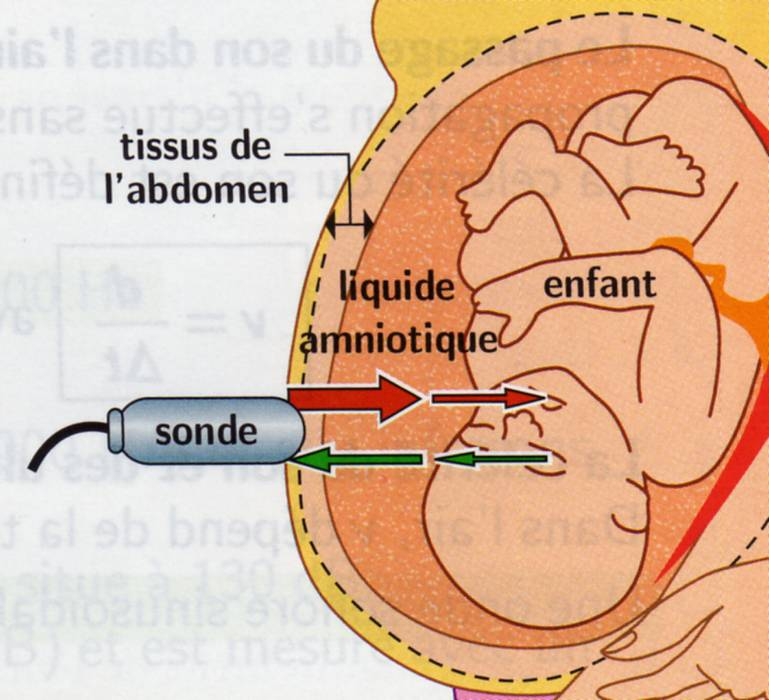
\includegraphics[width=5.009cm,height=4.621cm]{Pictures/1000000000000301000002BCCF7FB7734DEACB0A.jpg}

Un examen échographique est réalisé avec une sonde qui émet des
impulsions ultrasonores de fréquence 4 MHz. La vitesse des ondes dans le
milieu concerné est de 1540 m/s.

Cet examen fonctionne comme un sonar en numérisant à la fin le signal
réfléchi en image.

\begin{enumerate}
\def\labelenumi{\alph{enumi})}
\tightlist
\item
  Explique pourquoi on utilise des ultrasons plutôt que des ondes de
  plus petite fréquence
\end{enumerate}

\begin{enumerate}
\def\labelenumi{\alph{enumi})}
\tightlist
\item
  L'appareil décrit permet-il de détecter un embryon qui ne mesure que
  5mm~? Justifie ta réponse
\end{enumerate}

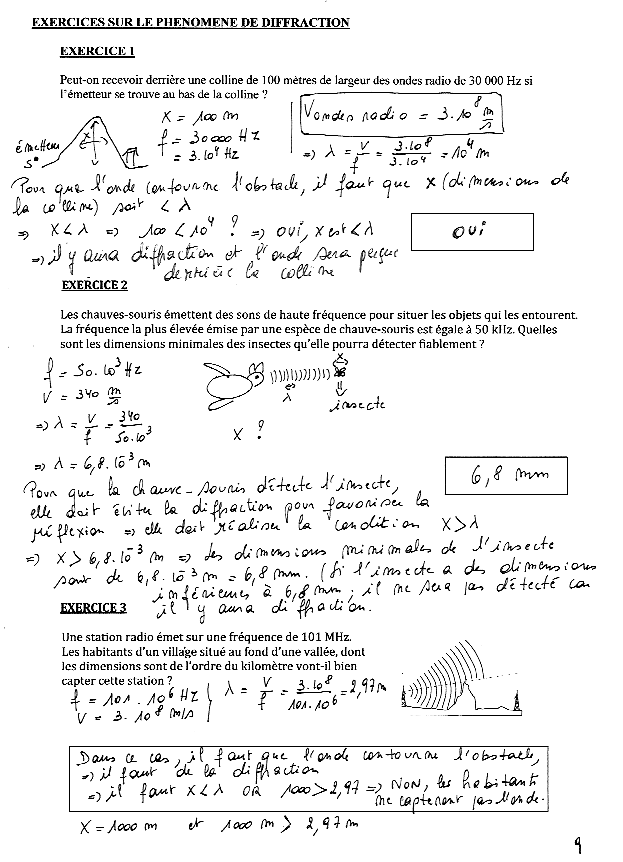
\includegraphics[width=18.503cm,height=25.615cm]{Pictures/100000010000026F0000035E638B1FB4AD6FDEB0.png}

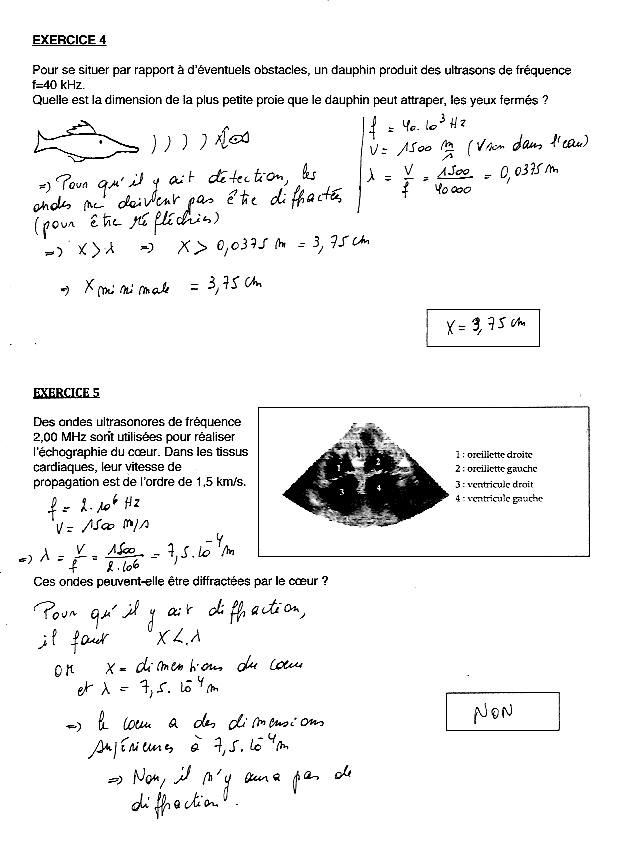
\includegraphics[width=18.503cm,height=25.476cm]{Pictures/10000001000002710000035C11CB153182C339CB.png}

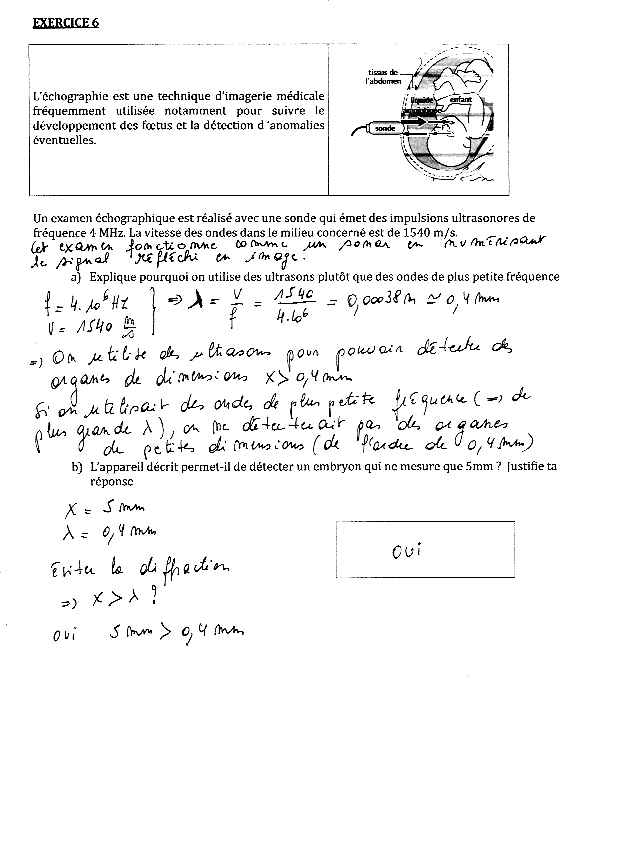
\includegraphics[width=18.503cm,height=25.476cm]{Pictures/10000001000002710000035C11584AA390113327.png}
